\documentclass[a4paper]{article}
\usepackage[noheadfoot, margin=3cm]{geometry}
\usepackage{graphicx}

\title{Stereo Vision using the OpenCV library}
\author{Sebastian Dr\"oppelmann \\ Moos Hueting \\ Sander Latour \\ Martijn van der Veen}
\date{June 2010}

\begin{document}

\graphicspath{{./images/}}

\begin{titlepage}
  \maketitle
\end{titlepage}

\section{Preface}
Stereo vision is one of the key subjects in the computer vision research. Stereo vision can be best described as taking two viewpoints in a 3D world, comparing the distance between the position of an object in both images and relating that to the distance of an object to the camera. Such information is retreived by a dense stereo algorithm of which the output is often a disparity depth map. A disparity depth map is a 2D image where the color of each pixel is directly linked to the distance of the pixel on that coordinate in the original image, in order words if an object is white it is depending on the implementation nearer or further away than a darker object. Our goal is to generate such a depth map from two images taken with two webcams.

Depthmaps are interesting because they can be used for various purposes: 
\begin{description}
 \item[3D modeling of 2D images] When you take two 2D images of a 3D enviroment and calculate the depthmap, you can create a 3D model of the scene by using the depth as the third dimension.
 \item[Tracking of objects] When you have a depthmap it is easier to track an object because you have additional segmentation possibilities. You can create segments of pixels that are near based on the depth of the pixels and their adjacency.
 \item[Recognising front objects] When you apply segmentation based on the depthmap, you can distinguish objects that are situated in the front of the scene.
 \item[As information about the environment in path planning] A depthmap supplies additional information for path planning.
\end{description}

\section{Practical problems}

\subsection{Webcams}
We will have to make the two webcams work on linux. Ideally we would have a live
feed from both webcams at all times.

\subsection{OpenCV}
We will have to get acquainted with the library OpenCV. See section
\ref{opencv}.

\section{Implementation}

\subsection{OpenCV}
\label{opencv}
OpenCV is a library of programming functions for real time computer vision. By using this library we can constrain our tasks to integrating various parts of OpenCV and expanding it where possible. If we would not use OpenCV, we would not have enough time to achieve our goal. OpenCV is a C library but has python binding which we will use to decrease the risk of programming errors.

\section{Theory}

\subsection{Epipolar geometry}
\label{epipolar}

\begin{figure}[h!]
  \label{fig:epipole}
  \centering
  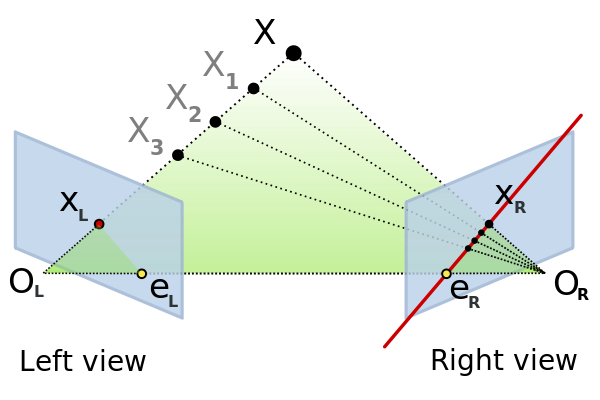
\includegraphics[width=1.0\textwidth]{Epipolar_geometry}
  \caption{All points $X_{1}, X_{2}, \cdots, X_{L}$ lie on the same epipolar line in the right view}
\end{figure}

Epipolar geometry is used in stereo vision to limit the searching space when
looking for matching points in both images. A point $X$ in 3D space is seen in
image $A$ as a point $x$, which is on the line between camera $A$'s focal point
and point $X$. This line is seen by camera $B$ as a line. This is called an
\emph{epipolar line}. Given both the cameras internal and external matrices and
a point $x_A$ we can generate an epipolar line corresponding to this point in
image $B$. This constrains the search space to this 1D line.

The points called $e_{L}$ and $e_{R}$ in figure \ref{fig:epipole} are called the
\emph{epipolar points} of both images. Epipolar lines rotate around the epipolar
point of a given image.

For more information on epipolar geometry, see \cite{Hartley2004}.

\subsection{Rectification}
\label{rectification}
As we have seen in section \ref{epipolar}, we can constrain the search space to
a 1D line. However due to the nature computers store images, it would be very
convenient if these epipolar lines were parallel to the horizontal scanlines.
This is done by a process called \emph{rectification}. This process transforms
both images so that the epipolar lines of the images align horizontally. For
this, we need a matrix that relates the two cameras. This matrix is called the
\emph{fundamental matrix} or \emph{bifocal tensor} and is denoted by the symbol
$F$.

\subsubsection{Fundamental matrix}
Given a point $x$ in image $A$, $Fx$ describes the epipolar line in image
$B$ on which the corresponding point $x'$ must lie. This means that $F$ has to
satisfy the equation
\[ x'^{T}Fx = 0 \]
for all corresponding points $x$ and $x'$. Given enough corresponding points, we
can solve this equation linearly. The more points available, the more accurate
this fundamental matrix becomes.\footnote{That is, if the corresponding points
are accurate as well.}

\subsubsection{Chessboard points}
The corresponding points necessary for generating the fundamental matrix is
obtained by making multiple pictures of a chessboard in the environment. The
OpenCV toolkit has a builtin function to recognize the corners of a chessboard.
In this project we will not elaborate on that subject.

\subsection{Dense stereo}
Dense stereo combines the two images you get from the rectification
and calculates the position of the pixels in the left image and
outputs where the pixel is located in the right image. With this method we
calculate the pixel's distance from the camera. 
The depth is then translated to a depth map where points closer
to the camera are almost white whereas points further away are almost
black. Points in between are shown in grayscale, which get darker
 the further away the point gets from the camera.

\begin{figure}
\centering
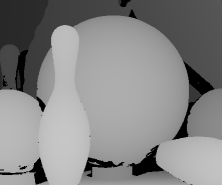
\includegraphics[width=0.3\textwidth]{depthmap}
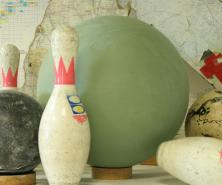
\includegraphics[width=0.3\textwidth]{depthmap_original}
\caption{A depthmap with the corresponding picture}
\end{figure}

To achieve this you have a whole list of algorithms that do
the trick.\footnote{A good overview can be found at
http://vision.middlebury.edu/stereo/eval/}

Most of these algorithms are based on 4 principles: 

\begin{itemize}
\item Graph Cut
\item Believe Propagation
\item Region Based
\item Dynamic Programming
\end{itemize}

These algorithms have to deal with the following problems in their
calculations:

\begin{itemize}
    \item Matching points in both images
    \item Occlusion
\end{itemize}

\subsubsection{Matching}
The main goal of such an algorithm is of matching one
point in one image to the corresponding point in the other image. During the
matching there are several tasks that the algorithm has to perform. At
first it has to compare the epipolar lines of the images pixel by
pixel. For every pixel on one line you have to find the counterpart on
the corresponding epipolar line in the other image. Often the pixels aren't
in the same order, for example if
there is a lamp pole in front of a house, things that lie on
the left side of the lamp pole in the left picture could sit on the right
side in the right picture.

\begin{figure}
\centering
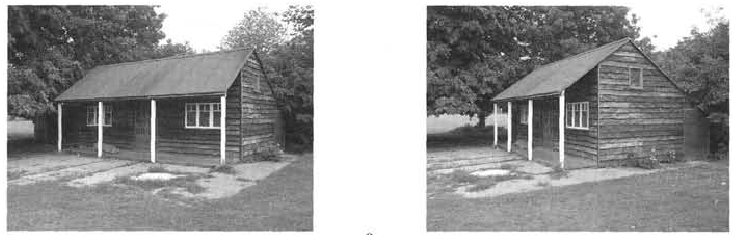
\includegraphics[width=0.8\textwidth]{matching_problems_direction}  
\caption{On the left image the window is completely on the left of the pole,
whereas in the right image, the window is completely on the right}
\end{figure}

Another problem is occlusion of the pixels. Some things that are
visible in one picture can be hidden behind objects in the other
picture. This has to be caught and handled.

\begin{figure}
\centering
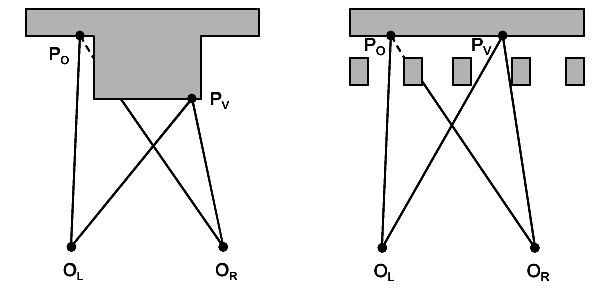
\includegraphics[width=0.8\textwidth]{matching_problems_occlusion}
\caption{Two examples of occlusion problems when working with stereo vision}
\end{figure}

Because the OpenCV library that we have chosen has the basic
implementation of a graph cut algorithm from Kolmogorov, we will start with
that specific algorithm.
It is a bit slow and not the best algorithm to handle occlusion but because it is
easy to use we will at first use this algorithm and later replace it
with a better working one.

\newpage
\section{Planning}
\begin{itemize}
  \item Week 1
    \begin{itemize}
      \item Reading literature
      \item Getting webcams to work
      \item Choosing dense algorithm
    \end{itemize}
  \item Week 2 and 3
    \begin{itemize}
      \item Implementing
        \begin{itemize}
          \item Dense disparity map algorithm
          \item Camera calibration using epipolar geometry
          \item Rectification of images
        \end{itemize}
      \item Halfway report
    \end{itemize}
  \item Week 4
    \begin{itemize}
      \item Optimizing and testing
      \item If there's enough time left
        \begin{itemize}
          \item Generate 3D image of environment
          \item Remove background using dense disparity map
        \end{itemize}
    \end{itemize}
\end{itemize}

\section{Tasks}
  \begin{itemize}
    \item Martijn and Moos
    \begin{itemize}
      \item Camera calibration
      \item Epipolar geometry
    \end{itemize}
    \item Sander and Sebastian
    \begin{itemize}
      \item Finding corresponding points
      \item Generating depth map
    \end{itemize}
  \end{itemize}

\bibliographystyle{plain}
\bibliography{verslag}

\end{document}
